\documentclass[10pt, landscape]{article}
\usepackage[scaled=0.92]{helvet}
\usepackage{calc}
\usepackage{multicol}
\usepackage[a4paper,margin=3mm,landscape]{geometry}
\usepackage{amsmath,amsthm,amsfonts,amssymb}
\usepackage{color,graphicx,overpic}
\usepackage{hyperref}
\usepackage{newtxtext} 
\usepackage{enumitem}
\usepackage[table]{xcolor}
\usepackage{mathtools}
\setlist{nosep}
% for including images
\graphicspath{ {./images/} }

\pdfinfo{
  /Title (CS3230.pdf)
  /Creator (TeX)
  /Producer (pdfTeX 1.40.0)
  /Author (Jovyn Tan)
  /Subject (CS3230)
/Keywords (CS3230, nus,cheatsheet,pdf)}

% Turn off header and footer
\pagestyle{empty}

% redefine section commands to use less space
\makeatletter
\renewcommand{\section}{\@startsection{section}{1}{0mm}%
  {-1ex plus -.5ex minus -.2ex}%
  {0.5ex plus .2ex}%x
{\normalfont\large\bfseries}}
\renewcommand{\subsection}{\@startsection{subsection}{2}{0mm}%
  {-1explus -.5ex minus -.2ex}%
  {0.5ex plus .2ex}%
{\normalfont\normalsize\bfseries}}
\renewcommand{\subsubsection}{\@startsection{subsubsection}{3}{0mm}%
  {-1ex plus -.5ex minus -.2ex}%
  {1ex plus .2ex}%
{\normalfont\small\bfseries}}%
\makeatother

\renewcommand{\familydefault}{\sfdefault}
\renewcommand\rmdefault{\sfdefault}
%  makes nested numbering (e.g. 1.1.1, 1.1.2, etc)
\renewcommand{\labelenumii}{\theenumii}
\renewcommand{\theenumii}{\theenumi.\arabic{enumii}.}
\renewcommand\labelitemii{•}
\renewcommand\labelitemiii{•}

\definecolor{mathblue}{cmyk}{1,.72,0,.38}
\everymath\expandafter{\the\everymath \color{mathblue}}

% Don't print section numbers
\setcounter{secnumdepth}{0}

\setlength{\parindent}{0pt}
\setlength{\parskip}{0pt plus 0.5ex}
%% adjust spacing for all itemize/enumerate
\setlength{\leftmargini}{0.5cm}
\setlength{\leftmarginii}{0.5cm}
\setlist[itemize,1]{leftmargin=2mm,labelindent=1mm,labelsep=1mm}
\setlist[itemize,2]{leftmargin=3mm,labelindent=1mm,labelsep=1mm}
\setlist[itemize,3]{leftmargin=3mm,labelindent=1mm,labelsep=1mm}

% adding my commands
\input{../commands/style-helpers.tex}
\input{../commands/code.tex}
\newcommand{\Mod}[1]{\ (\mathrm{mod}\ #1)}

% -----------------------------------------------------------------------

\begin{document}
\raggedright
\footnotesize
\begin{multicols*}{4}
  % multicol parameters
  \setlength{\columnseprule}{0.25pt}

  \begin{center}
    \fbox{%
      \parbox{0.8\linewidth}{\centering \textcolor{black}{
          {\Large\textbf{CS3230}}
        \\ \normalsize{AY21/22 SEM 2}}
        \\ {\footnotesize \textcolor{gray}{github/jovyntls}}
      }%
    }
  \end{center}

  \section{01. COMPUTATIONAL MODELS}

  \begin{itemize}
    \item \definition{algorithm} a well-defined procedure for finding the correct solution to the input
    \item \textbf{correctness}
      \begin{itemize}
        \item \definition{worst-case correctness} correct on \textit{every valid input}
        \item other types of correctness: correct on random input/with high probability/approximately correct
      \end{itemize}
    \item \textbf{efficiency} / \definition{running time} measures the number of steps executed by an algorithm as a function of the \textit{input size} (depends on computational model used)
      \begin{itemize}
        \item number input: typically the length of binary representation
        \item \definition[running time]{worst-case} \textit{max} number of steps executed when run on an input of size $n$ 
      \end{itemize}
  \end{itemize}

  \begin{fixedbox}[0.9]
    \definition{adversary argument} 
    \\ inputs are decided such that they have different solutions
  \end{fixedbox}

  \subsection{Comparison Model}

  \begin{itemize}
    \item algorithm can \textbf{compare} any two elements in one time unit ($x>y$, $x<y$, $x=y$)
    \item running time = number of pairwise comparisons made
    \item array can be manipulated at no cost
  \end{itemize}

  \subsubsection{Decision Tree}

  \begin{itemize}
    \item each comparison represents the relationship between two elements
    \item each node is a comparison
    \item each branch is an outcome of the comparison
    \item log base is determined by the number of branches per node
    \item each leaf is a class label (decision after \textit{all} comparisons)
    \item \textbf{lower bound of worst-case} runtime = height of tree
    \item \# of leaves = \# of permutations $\Rightarrow \lg(n!) = \Theta(n \lg n)$ 
    \item any decision tree that can sort $n$ elements must have height $\Omega (n \lg n)$.
  \end{itemize}

  \subsubsection{\texttt{Max} Problem}

  \textit{problem}: find largest element in array $A$ of $n$ distinct elements

  \begin{niceproof}
    $n-1$ comparisons are needed

    fix an algorithm $M$ that solves the \texttt{Max} problem on all inputs using $< n-1$ comparisons. construct graph $G$ where nodes $i$ and $j$ are adjacent iff $M$ compares $i$ \& $j$.
    \\* \includegraphics[width=0.9\linewidth]{cs3230-maximum-problem-graph.png} 

    $M$ cannot differentiate $A$ and $A'$.
  \end{niceproof}

  \subsubsection{Second Largest Problem}

  \textit{problem}: find the second largest element in $<2n-3$ comparisons (2x Maximum $\Rightarrow$ $\scriptstyle (n-1) + ((n-1)-1) = 2n-3$ )

  \begin{itemize}
    \item \textit{solution}: \textbf{knockout tournament} $\Rightarrow n + \lceil \lg n \rceil - 2$
      \\* \includegraphics[width=0.8\linewidth]{cs3230-second-largest-solution.png} 
      \begin{enumerate}
        \item bracket system: $n-1$ matches 
          \begin{itemize}
            \item every non-winner has lost exactly once
          \end{itemize}
        \item then compare the elements that have lost to the largest
          \begin{itemize}
            \item the 2nd largest element must have lost to the winner
            \item compares $\lceil \lg n \rceil$ elements that have lost to the winner using $\lceil \lg n \rceil -1$ comparisons 
          \end{itemize}
      \end{enumerate}
  \end{itemize}

  \subsubsection{Sorting}

  \textit{Claim.} there is a sorting algorithm that requires $\leq n \lg n - n + 1$ comparisons.

  \begin{niceproof}
    every sorting algorithm must make $\geq \lg (n!)$ comparisons.
  \end{niceproof}

  \begin{enumerate}
    \item let set $\mathcal{U}$ be the set of all permutations of the set $\{1, \dots, n\}$ that the adversary could choose as array $A$. $\vert \mathcal{U} \vert = n!$ 
    \item for each query "is $A_i > A_j$?", 
      \\* if $\mathcal{U}_{yes} = \{A \in \mathcal{U} : A_i > A_j\}$ is of size $\geq \vert\mathcal{U}\vert /2$, set $\mathcal{U} := \mathcal{U}_{yes}$. else: $\mathcal{U} := \mathcal{U} \backslash \mathcal{U}_{yes}$
    \item the size of $\mathcal{U}$ decreases by at most half with each comparison
    \item with $< \lg (n!)$ comparisons, $\mathcal{U}$ will still contain at least 2 permutations
  \end{enumerate}

  \begin{tightcenter}
    $n! \geq (\frac{n}{e})^n$ 
    \\* $\Rightarrow \lg (n!) \geq n \lg (\frac{n}{e}) = n \lg n - n \lg e$
    \\* $\approx n \lg n - 1.44n$
    \\* $\Rightarrow$ roughly $n \lg n$ comparisons are \textbf{required} and \textbf{sufficient} for sorting $n$ numbers
  \end{tightcenter}

  \subsection{String Model}

  \begin{tightcenter}
    \begin{tabular}{|c|l|}
      \hline
      input & string of $n$ bits \\\hline
      each query & find out \textbf{one bit} of the string \\ \hline
    \end{tabular}
  \end{tightcenter}

  \begin{itemize}
    \item $n$ queries are \textbf{necessary} and \textbf{sufficient} to check if the input string is all 0s.
    \item \definition{query complexity} number of bits of the input string queried by the algorithm
    \item \definition{evasive} a problem requiring $n$ query complexity
  \end{itemize}

  \subsection{Graph Model}

  \begin{tightcenter}
    \begin{tabular}{|c|p{0.7\linewidth}|}
      \hline
      input & (symmetric) adjacency matrix of an $n$-node undirected graph \\\hline
      each query & find out if an edge is present between two chosen nodes (one entry of $G$) \\\hline
    \end{tabular}
  \end{tightcenter}

  \begin{itemize}
    \item \definition{evasive} requires $\binom{n}{2}$ queries
    \item \textit{Proof}. determining whether the graph is connected is evasive (requires $\binom{n}{2}$ queries) 
      \begin{enumerate}
        \item suppose $M$ is an algorithm making $\leq \binom{n}{2}$ queries.
        \item whenever $M$ makes a query, the algorithm tries not adding this edge, but adding all remaining unqueried edges. 
          \begin{enumerate}
            \item if the resulting graph is connected, $M$ replies $0$ (i.e. edge does not exist)
            \item else: replies $1$ (edge exists)
          \end{enumerate}
        \item after $< \binom{n}{2}$ queries, at least one entry of the adjacency matrix is unqueried.
      \end{enumerate}
      \qed
  \end{itemize}


  \section{02. ASYMPTOTIC ANALYSIS}

  \begin{itemize}
    \item \definition{algorithm} a \textit{finite} sequence of well-defined instructions to solve a given computational problem
    \item \definition{word-RAM model} runtime is the total number of instructions executed
      \begin{itemize}
        \item operators, comparisons, if, return, etc
        \item each instruction operates on a \textit{word} of data (limited size) $\Rightarrow$ fixed constant amount of time
      \end{itemize}

  \end{itemize}

  \subsection{Asymptotic Notations}

  \begin{tightcenter}
    \textbf{upper bound ($\leq$)}: $f(n) = O(g(n))$
    \\* if $\exists c>0, n_0>0$ such that $\forall n \geq n_0$, 
    \begin{tightbox}
      $0 \leq f(n) \leq cg(n)$
    \end{tightbox}
    

    \ \\ \textbf{lower bound ($\geq$)}: $f(n) = \Omega(g(n))$
    \\* if $\exists c>0, n_0>0$ such that $\forall n \geq n_0$, 
    \begin{tightbox}
      $0 \leq cg(n) \leq f(n)$
    \end{tightbox}

    \ \\ \textbf{tight bound}: $f(n) = \Theta(g(n))$
    \\* if $\exists c_1, c_2, n_0>0$ such that $\forall n \geq n_0,$
    \begin{tightbox}
      $0 \leq c_1 g(n) \leq f(n) \leq c_2 g(n)$ 
    \end{tightbox}

    \ \\ \textbf{$o$-notation ($<$)}: $f(n) = o(g(n))$
    \\* if $\forall c>0, \exists n_0>0$ such that $\forall n \geq n_0$, 
    \begin{tightbox}
      $0 \leq f(n) < cg(n)$
    \end{tightbox}

    \ \\ \textbf{$\omega$-notation ($>$)}: $f(n) = \omega(g(n))$
    \\* if $\forall c>0, \exists n_0>0$ such that $\forall n \geq n_0$, 
    \begin{tightbox}
      $0 \leq cg(n) < f(n)$
    \end{tightbox}
  \end{tightcenter}

  \begin{niceproof}
    $(n+1)! \ne O(n!)$ since $\frac{(n+1)!}{n!}=(n+1)>c$
  \end{niceproof}

  \subsection{Limits}

  Assume $f(n), g(n) > 0$.
  \begin{align*}
    &\lim\limits_{n \to \infty} \frac{f(n)}{g(n)} = 0 &\Rightarrow f(n) = o(g(n)) \\
    &\lim\limits_{n \to \infty} \frac{f(n)}{g(n)} < \infty &\Rightarrow f(n) = O(g(n)) \\
    0 < &\lim\limits_{n \to \infty} \frac{f(n)}{g(n)} < \infty &\Rightarrow f(n) = \Theta(g(n)) \\
        &\lim\limits_{n \to \infty} \frac{f(n)}{g(n)} > 0 &\Rightarrow f(n) = \Omega(g(n)) \\
        &\lim\limits_{n \to \infty} \frac{f(n)}{g(n)} = \infty &\Rightarrow f(n) = \omega(g(n))
  \end{align*}

  \begin{niceproof}
    \begin{enumerate}
      \item Since $\lim_{n \to \infty} = 0$, we have for all $\epsilon>0$, there exists $\delta>0$ s.t $\frac{f(n)}{g(n)}<\epsilon$ for $n>\delta$
      \item Set $c=\epsilon$ and $n_0=\delta$
      \item $\forall n \geq n_0$, $\frac{f(n)}{g(n)}<$c 
      \item $\forall n \geq n_0$, $f(n) < cg(n)$ 
     \item By definition, f(n)=o(g(n))
    \end{enumerate}
  \end{niceproof}

  \subsection{Properties of Big O}

  \begin{fixedbox}
    $\Theta(g(n)) = O(g(n)) \cap \Omega(g(n))$
  \end{fixedbox}

  \begin{itemize}
    \item \textbf{transitivity} - applies for $O, \Theta, \Omega, o, \omega$
      $f(n) = O(g(n)) \land g(n) = O(h(n)) \Rightarrow f(n) = O(h(n))$ 
    \item \textbf{reflexivity} - for $O, \Omega, \Theta, \quad f(n) = O(f(n))$ 
    \item \textbf{symmetry} - $f(n) = \Theta(g(n)) \iff g(n) = \Theta(f(n))$
    \item \textbf{complementarity} - 
      \begin{itemize}
        \item $f(n) = O(g(n)) \iff g(n) = \Omega(f(n))$
        \item $f(n) = o(g(n)) \iff g(n) = \omega(f(n))$
      \end{itemize}
    \item \textbf{misc}
      \begin{itemize}
        \item if $f(n) = \omega(g(n))$, then $f(n) = \Omega(g(n))$
        \item if $f(n) = o(g(n))$, then $f(n) = O(g(n))$
      \end{itemize}
  \end{itemize}

  \begin{fixedbox}[0.8]
    $\log\log n < \log n < (\log n)^k < n^k < (n+1)!< k^n$
  \end{fixedbox}

  insertion sort: $O(n^2)$ with worst case $\Theta(n^2)$

  \section{03. ITERATION, RECURSION, DIVIDE-AND-CONQUER}

  \subsection{Iterative Algorithms}

  \begin{itemize}
    \item \definition{iterative} loop(s), sequentially processing input elements
    \item \textbf{loop invariant} implies correctness if 
      \begin{itemize}
        \item \textit{initialisation} - true before the first iteration of the loop
        \item \textit{maintenance} - if true before an iteration, it remains true at the beginning of the next iteration
        \item \textit{termination} - true when the algorithm terminates
      \end{itemize}
  \end{itemize}

  \subsubsection{examples}

  \begin{itemize}
    \item \textbf{insertionSort}: with loop variable as $j$, $A[1..J-1]$ is sorted.
    \item[] \begin{enumerate}
      \item A[1...i]=A'[1...i]. Elements not considered are unaffected.
      \item A[i+2...j]=A'[i+1...j-1]. Relative order of shifted elements is preserved.
      \item A[i+2...j] $>$key. Elements to its right are sorted and greater.
    \end{enumerate}
    \item \textbf{selectionSort}: with loop variable as $j$, the array $A[1..j-1]$ is sorted and contains the $j-1$ smallest elements of $A$.
    % \item \textbf{Misra-Gries algorithm} (determines which bit occurs more in an $n$-bit array $A$):
    %   \begin{itemize}
    %     \item if there is an equal number of 0's and 1's, then $id=\bot$ and $count = 0$
    %     \item if $z \in \{0, 1\}$ is the majority element, then $id=z$ and $count$ equals the difference between the count of the bits.
    %   \end{itemize}

    \item \textbf{Dijkstra's}:
    \item[] \begin{niceproof} 
      \begin{enumerate}
        \item \textbf{invariant 1}$\forall x \in R$: $dist[x] = \sigma(s,x)$
        \item \textbf{invariant 2}$\forall$ y neighbouring $x\in R$: $dist[y]=min_{x\in R}\sigma(s,x)+W(x,y)$
      \end{enumerate}
    \end{niceproof}
  \end{itemize}

\subsection{Recursive Algorithm}
\begin{itemize}
  \item \definition{recursive} solves sub problems
  \item Correctness is proven using \textbf{mathematical induction} on size of problem
  \item Use strong induction, prove base case, show algorithm works assuming it works for all smaller cases
\end{itemize}

\subsection{Examples}
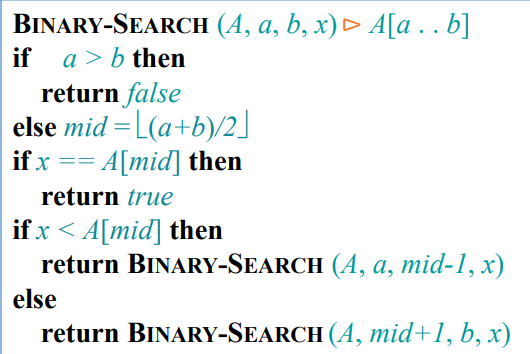
\includegraphics[width=0.9\linewidth]{binary_search.png} \\

\begin{itemize}
  \item \textbf{binary search}(A,a,b,x) returns the correct answer when b-a+1=n
  \item Base case: n=b-a+1=0, since a=b+1, A[a..b] is empty and the answer is false
  \item Inductive step: $n=b-a+1 > 0$
  \item By strong induction, assume (A,a',b',x) returns the correct answer for all $j$ s.t $0\le j\le n-1$ where $j=b'-a'+1$
  \item By the algorithm, $mid=\lfloor \frac{a+b}{2} \rfloor$ and $a\le mid\le b$
  \item If $x==A[mid]$ then $x \in A[a..b]$ and the algorithm returns true correctly
  \item If $x<A[mid]$ then $x \in A[a..mid-1] iff x\in A[a..b]$ 
  \item By the inductive hypothesis, (A,a,mid-1,x) is correct since $0\le (mid-1)-a+1=mid-a\le n-1$
  \item The $x>A[mid]$ is similar
\end{itemize}


  \subsection{Divide-and-Conquer}

  \subsubsection{powering a number}

  \textit{problem:} compute $f(n, m) = a^n\Mod{m}$ for all $n, m \in \mathbb{Z}$

  \begin{itemize}
    \item observation: $f(x+y, m) = f(x, m) * f(y, m) \Mod{m}$
    \item \textbf{naive solution}: recursively compute and combine $f(n-1, m) * f(1, m) \Mod m$ 
      \begin{itemize}
        \item $T(n) = T(n-1) + T(1) + \Theta(1) \Rightarrow T(n) = \Theta (n)$
      \end{itemize}
    \item \textbf{better solution}: divide and conquer (only one sub problem computed)
      \begin{itemize}
        \item divide: trivial
        \item conquer: recursively compute $f(\lfloor n / 2 \rfloor, m)$ 
        \item combine: 
          \begin{itemize}
            \item $f(n, m) = f(\lfloor n / 2 \rfloor, m)^2 \Mod m$ if n is even
            \item $f(n, m) = f(1, m) * f(\lfloor n / 2 \rfloor, m)^2 \Mod m$ if odd
          \end{itemize}
        \item $T(n) = T(n/2) + \Theta(1) \Rightarrow \Theta(\log n)$
      \end{itemize}
  \end{itemize}

    \subsubsection{Peak finding}
  \textit{problem:} Find the peak element (no neighbours are greater) in 2D array 

\begin{itemize}
    \item \textbf{\textit{Naive}} O(mn)
    \item[] \begin{itemize}
      \item for the middle column, find the maximum element
      \item return if it is peak
      \item p1=Find2DPeak(left)
      \item p2=Find2DPeak(right)
      \item return p1 or p2 if one is a peak
    \end{itemize}
    \item \textbf{\textit{Divide and conquer}} O(mlogn), $T(n)=T(n/2)+O(1)$ n is number of columns 
    \item \begin{itemize}
      \item find the middle column, find the maximum element
      \item if it is a peak, return it
      \item if not, recurse on the side with a larger element
    \end{itemize}
    \item \textbf{\textit{Optimised}} O(m+n)
    \item[] 
    \begin{itemize}
      \item find the middle column, find the maximum element
      \item recurse on the quarter with the larger element
    \end{itemize}
  \end{itemize}


  \section{Solving Recurrences}

  for $a$ sub-problems of size $\frac{n}{b}$ where $f(n)$ is the time to divide and combine, 
  \begin{tightcenter}
    $T(n) = aT(\frac{n}{b}) + f(n)$
  \end{tightcenter}


  \subsection{Telescoping}
  Express $\frac{T(n)}{g(n)} as \frac{T(\frac{n}{b})}{g(\frac{n}{b})} + h(n)$ \\
  Choose the poly(n) part of f(n) as $\frac{f(n)}{b}$
  \begin{enumerate}
    \item Example: T(n) = 2T(n/2) + n
    \item $\frac{T(n)}{n}=\frac{T(n/2)}{n/2}+1$
  \end{enumerate}
  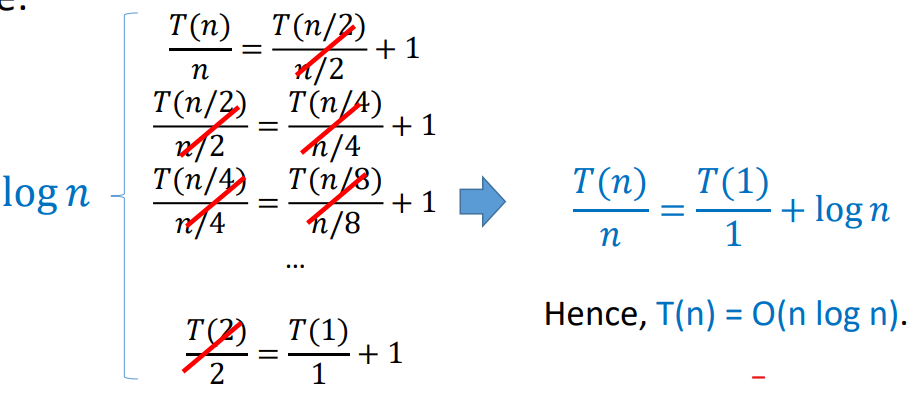
\includegraphics[width=0.9\linewidth]{telescoping.png} \\

  If g(n)=n, we need a=b since g(n) = $n^{\log_b(a)}$

  \subsection{Recursion tree}

  total = height $\times$ number of leaves

  \begin{itemize}
    \item each node represents the cost of a single subproblem
    \item height of the tree = longest path from root to leaf
  \end{itemize}

  \begin{tightcenter}
    \includegraphics[width=0.9\linewidth]{cs3230-recursion-tree-example-1.png} 
    \includegraphics[width=0.6\linewidth]{cs3230-recursion-tree-example-2.png} 
  \end{tightcenter}

  \subsection{Master method}

  \begin{itemize}
    \item  $a \geq 1, b > 1,$ and $f$ is asymptotically positive.
    \item a (number of sub problems), b(size of sub problems), f(time to divide and combine)
  \end{itemize} 

  \begin{math}
    T(n) = aT(\frac{n}{b}) + f(n) = \begin{cases}
      \Theta(n^{\log_ba}) & \text{ if } f(n) < n^{\log_ba} \text{ polynomially}
      \\ \Theta(n^{\log_ba} \log n) & \text{ if } f(n) = n^{\log_ba} 
      \\ \Theta(f(n)) & \text{ if } f(n) > n^{\log_ba} \text{ polynomially}
    \end{cases}
  \end{math}

  \subsubsection{three common cases}

  \begin{enumerate}
    \item If $f(n) = O(n^{\log_b a-\epsilon})$ for some constant  $\epsilon > 0$, 
      \begin{itemize}
        \item $f(n)$ grows polynomially slower than $n^{\log_ba}$ by $n^\epsilon$ factor.
        \item then $T(n) = \Theta(n^{\log_ba})$.
        \item This is when overhead at leaf $>$ overhead at root
      \end{itemize}
    \item If $f(n) = \Theta(n^{\log_ba} \log^kn) $ for some $k \geq 0$,
      \begin{itemize}
        \item $f(n)$ and $n^{\log_ba}$ grow at similar rates.
        \item then $T(n) = \Theta(n^{\log_ba}\log^{k+1} n)$
      \end{itemize}
    \item If $f(n) = \Omega(n^{\log_ba + \epsilon})$ for some constant $\epsilon > 0$, 
      \begin{itemize}
        \item and $f(n)$ satisfies the \textbf{regularity condition} 
          \begin{itemize}
            \item $af(n/b) \leq cf(n)$ for some constant $c<1$ and \\* all sufficiently large $n$
            \item this guarantees that the sum of subproblems is smaller than $f(n)$.
          \end{itemize} 
        \item $f(n)$ grows polynomially faster than $n^{\log_ba}$ by $n^\epsilon$ factor
        \item then $T(n) = \Theta(f(n))$.
        \item This is when the root (splitting) $>$ leaf
      \end{itemize}
  \end{enumerate}

  \subsection{Substitution method}

  \begin{enumerate}
    \item guess that $T(n) = O(f(n))$. 
    \item verify by induction:
      \begin{enumerate}
        \item to show that for $n \geq n_0$, $T(n) \leq c \cdot f(n)$
        \item set $c = \max\{2, q\}$ and $n_0 = 1$
        \item verify base case(s): $T(n_0) = q$
        \item recursive case ($n > n_0$):
          \begin{itemize}
            \item by strong induction, assume $T(k) \leq c \cdot f(k)$ for $n > k \geq n_0$
            \item T(n) = <recurrence> ... $\leq c \cdot f(n)$
          \end{itemize}
        \item hence $T(n) = O(f(n))$.
      \end{enumerate}
  \end{enumerate}
  \attention may not be a tight bound!

  \subsubsection{example}

  \begin{niceproof}
    $T(n) = 4T(n/2) + n^2/\lg n \Rightarrow \Theta(n^2\lg \lg n)$

    $T(n) = 4T(n/2) + \frac{n^2}{\lg n}$ \\
    $= 4( 4T(n/4) + \frac{(n/2)^2}{\lg n - lg 2} ) + \frac{n^2}{\lg n}$ \\ 
    $= 16 T(n/4) + \frac{n^2}{\lg n - \lg 2} + \frac{n^2}{\lg n}$ \\
    $= \sum\limits^{\lg n}_{k=1} \frac{n^2}{\lg n - k}$ \\
    $= n^2 \lg \lg n$ by approx. of harmonic series ($\sum\frac{1}{k}$) \\

    Can also be solved via telescoping using g(n)=$n^2$
  \end{niceproof}

  \begin{niceproof}
    $T(n) = 4T(n/2) + n \Rightarrow O(n^2)$

    To show that for all $n \geq n_0$, $T(n) \leq c_1n^2 - c_2n$

    1. Set $c_1 = q+1, c_2 = 1, n_0 = 1$. 

    2. Base case ($n=1$): subbing into $c_1n^2 - c_2n$,
    $T(1) = q \leq (q+1)(1)^2 - (1)(1)$ 

    3. Recursive case ($n>1$):
    \begin{itemize}
      \item by strong induction, assume $T(k) \leq c_1 \cdot k^2 - c_2 \cdot k$ for all $n>k \geq 1$ 
      \item $T(n) = 4T(n/2) + n$ 
        \\* $\quad\quad = 4(c_1 (n/2)^2 - c_2(n/2)) + n$
        \\* $\quad\quad = c_1n^2 - 2c_2n + n $
        \\* $\quad\quad = c_1n^2 - c_2n + (1-c_2) n$
        \\* $\quad\quad = c_1n^2 - c_2n \quad $ since $c_2=1 \Rightarrow 1-c_2 = 0$
        \\* \qed
    \end{itemize}
  \end{niceproof}
  
  \section{Non-comparison sort}
  \subsection{Counting sort}
  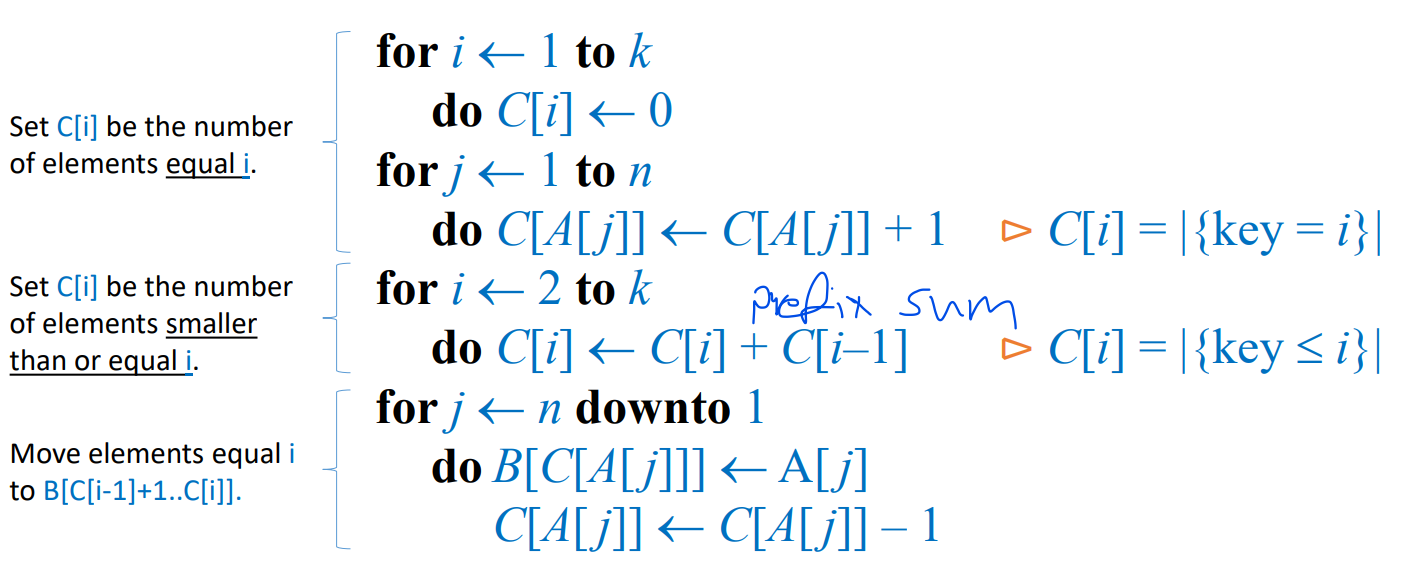
\includegraphics[width=0.95\linewidth]{counting_sort.png} 

  \begin{itemize}
    \item O(n+k), where k is the number of elements
    \item Stable 
  \end{itemize}

  \subsection{Radix sort}
  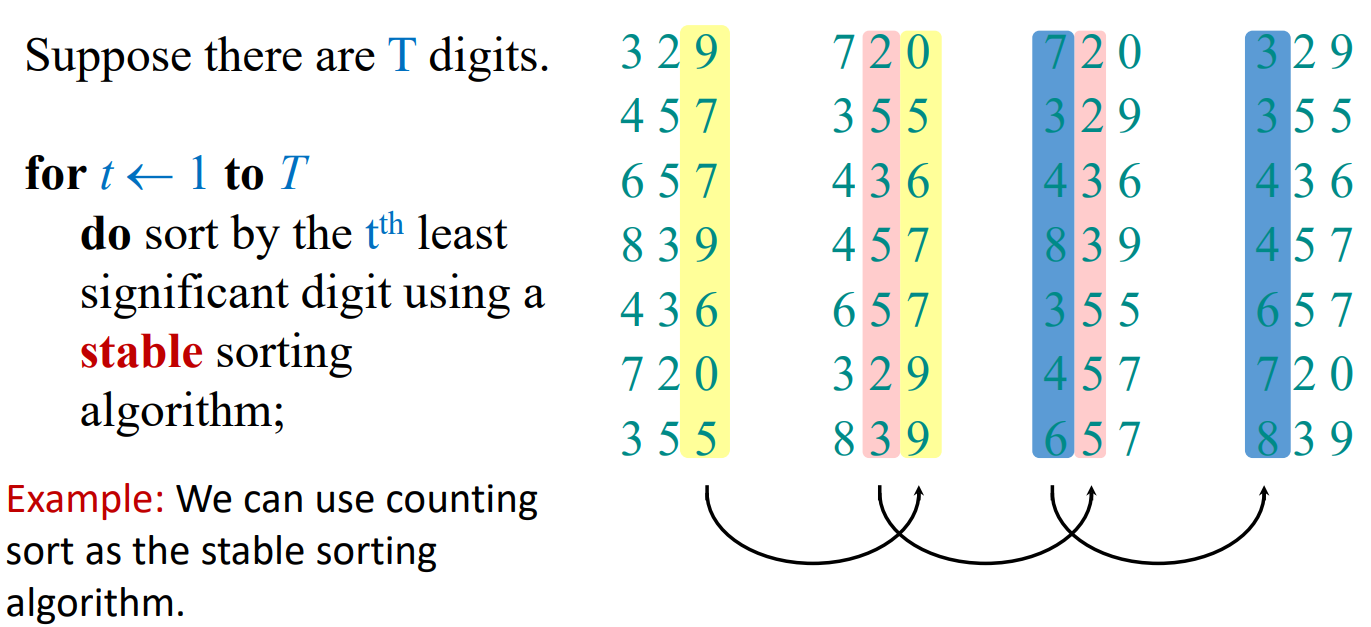
\includegraphics[width=0.95\linewidth]{radix_sort.png}
  \begin{itemize}
    \item Each pass processes r digits at $O(n+2^r)$
    \item $T(n,b)=\theta(\frac{b}{2}(n+2^r))$ where $b$ is the number of bits in the key
    \item Optimal r=$\lg n$ T(n,b)=$\theta(\frac{bn}{\lg n})$
    \item Fast when the number of passes ($\frac{b}{r}$) is small
    \item Little locality of reference, not cache friendly
  \end{itemize}

  \section{04. AVERAGE-CASE ANALYSIS \& RANDOMISED ALGORITHMS}

  \begin{itemize}
    \item \definition[$A(n)$]{average case} expected running time when the input is chosen uniformly at random from the set of all $n!$ permutations
      \begin{itemize}
        \item $A(n) = \frac{1}{n!} \sum_\pi Q(\pi)$ where $Q(\pi)$ is the time complexity when the input is permutation $\pi$.
        \item $A(n) = \mathop{\mathbb{E}}\limits_{x \sim \mathcal{D}_n} [ \text{Runtime of Alg on }x ] $
          \begin{itemize}
            \item $ \mathbb{E}_{x \sim \mathcal{D}_n} $ is a probability distribution on $U$ restricted to inputs of size $n$.
          \end{itemize}
      \end{itemize}
  \end{itemize}

  \subsection{Quicksort Analysis}

  \begin{itemize}
    \item divide \& conquer, linear-time $\Theta(n)$ partitioning subroutine
    \item assume we select the first array element as pivot 
    \item $T(n) = T(j) + T(n-j-1) + \Theta(n)$
      \begin{itemize}
        \item if the pivot produces subarrays of size $j$ and $(n-j-1)$
      \end{itemize}
    \item \textbf{worst-case}: $T(n) = T(0) + T(n-1) + \Theta(n) \Rightarrow \Theta(n^2)$ 
  \end{itemize}

  \begin{niceproof}
    for quicksort, $A(n) = O(n \log n)$

    let $P(i)$ be the set of all those permutations of elements $\{e_1, e_2, \dots, e_n\}$ that begins with $e_i$.

    Let $G(n, i)$ be the average running time of quicksort over $P(i)$.
    Then $G(n) = A(i-1) + A(n-i) + (n-1)$.
    $A(n) = \frac{1}{n} \sum_{i=1}^n G(n, i)$
    \\ $\quad\quad = \frac{1}{n} \sum_{i=1}^n ( A(i-1) + A(n-i) + (n-1) )$
    \\ $\quad\quad = \frac{2}{n} \sum_{i=1}^n A(i-1)+n-1$
    \\ $\quad\quad = O(n\log n)$ by taking it as area under integration
  \end{niceproof}

  \subsubsection{quicksort vs mergesort}

  \begin{center}
    \begin{tabular}{|c|c|c|c|}
      \hline
      & average & best & worst \\\hline
      quicksort & $1.39n\lg n$ &  $n \lg n$ & $n(n-1)$ \\\hline
      mergesort & $n\lg n$ &  $n \lg n$ & $n \lg n$ \\\hline
    \end{tabular}
  \end{center}

  \begin{itemize}
    \item disadvantages of mergesort:
      \begin{itemize}
        \item overhead of temporary storage
        \item cache misses
      \end{itemize}
    \item advantages of quicksort
      \begin{itemize}
        \item in place
        \item reliable (as $n \uparrow$, chances of deviation from avg case $\downarrow$)
      \end{itemize}
    \item issues with quicksort
      \begin{itemize}
        \item \definition{distribution-sensitive} time taken depends on the initial (input) permutation. Resolved with median pivot or randomised partitions
      \end{itemize}
  \end{itemize}

  \subsection{Randomised Algorithms}

  \begin{itemize}
    \item \definition{randomised algorithms} output and running time are \textbf{functions} of the \textbf{input} and \textbf{random bits chosen}
      \begin{itemize}
        \item vs non-randomised: output \& running time are functions of the \textit{input only}
      \end{itemize}
    \item expected running time = worst-case running time = 
      \\* $E(n) = \max\limits_{ \text{input $x$ of size $n$} } \mathbb{E} [ \text{Runtime of RandAlg on }x ] $
    \item \textbf{randomised quicksort}: choose pivot at random 
      \begin{itemize}
        \item probability that the runtime of \textit{randomised} quicksort exceeds average by $x\% = n^{-\frac{x}{100}\ln\ln n}$ 
        \item P(time takes at least double of the average) = $10^{-15}$
        \item distribution insensitive
      \end{itemize}
  \end{itemize}

  \subsection{Balls into bins - Indicator Random Variable}
  There are $n$ balls and $m$ bins. Each ball is placed into a bin at random. How many empty bins? \\
  \begin{itemize}
    \item $X_i$ = 1 if ball $i$ is in bin $j$, 0 otherwise
    \item $E(X_i)=1*P(i^{th} bin_{empty}) + 0*P(...)$=$(1-\frac{1}{n})^m$
    \item $E(X)=E(X_1)+E(X_2)+..+E(X_n)=n(1-\frac{1}{n})^m$
  \end{itemize}


  \subsubsection{Randomised Quicksort Analysis}

  $T(n) = n-1 + T(q-1) + T(n-q)$

  Let $A(n) = \mathbb{E}[T(n)]$ where the expectation is over the randomness in expectation.

  Taking expectations and applying linearity of expectation:
  $A(n) = n-1 + \frac{1}{n} \sum^n_{q=1} (A(q-1) + A(n-q)) $ 
  $\;\quad\quad = n-1 + \frac{2}{n} \sum\limits^{n-1}_{q=1} A(q) $ 

  $A(n) = n \log n \quad \Rightarrow$ same as average case quicksort


  \subsubsection{Randomised Quickselect}

  \begin{itemize}
    \item $O(n)$ to find the $k^{th}$ smallest element
    \item randomisation: unlikely to keep getting a bad split
  \end{itemize}

  \subsubsection{Types of Randomised Algorithms}

  \begin{itemize}
    \item randomised \textbf{Las Vegas} algorithms
      \begin{itemize}
        \item output is always correct
        \item runtime is a \textit{random variable} 
        \item e.g. randomised quicksort, randomised quickselect
      \end{itemize}
    \item randomised \textbf{Monte Carlo} algorithms
      \begin{itemize}
        \item output may be incorrect with some small probability
        \item runtime is \textit{deterministic}
      \end{itemize}
  \end{itemize}

  \textbf{Examples}
  \begin{itemize}
    \item \textit{smallest enclosing circle:} given $n$ points in a plane, compute the smallest radius circle that encloses all $n$ points
      \begin{itemize}
        \item best \textbf{deterministic} algorithm: $O(n)$, but complex
        \item Las Vegas: average $O(n) $, simple solution
      \end{itemize}
    \item \textit{minimum cut:} given a connected graph $G$ with $n$ vertices and $m$ edges, compute the smallest set of edges whose removal would disconnect $G$.
      \begin{itemize}
        \item best \textbf{deterministic} algorithm: $O(mn)$
        \item \textbf{Monte Carlo}: $O(m \log n) $, error probability $n^{-c}$ for any $c$
      \end{itemize}
    \item \textit{primality testing:} determine if an $n$ bit integer is prime
      \begin{itemize}
        \item best \textbf{deterministic} algorithm: $O(n^6)$
        \item \textbf{Monte Carlo}: $O(kn^2)$, error probability $2^{-k}$ for $k$ checks
      \end{itemize}
  \end{itemize}

  \subsection{Geometric Distribution}

  Let $X$ be the number of trials repeated until success. 

  $X$ is a random variable and follows a geometric distribution with probability $p$.

  \begin{tightcenter}
    Expected number of trials, $E[X] = \frac{1}{p} $
    \\* $ Pr[X=k] = q^{k-1}p $
  \end{tightcenter}

  \subsubsection{Linearity of Expectation}

  For any two events $ X, Y $ and a constant $ a $, 
  \begin{tightcenter}
    $ E[X+Y] = E[X] + E[Y] $
    \\ $ E[aX] = aE[X] $
  \end{tightcenter}

  \subsubsection{Coupon Collector Problem}

  \textit{$ n $ types of coupon are put into a box and randomly drawn with replacement.
  What is the expected number of draws needed to collect at least one of each type of coupon?}

  \begin{itemize}
    \item let $ T_i $ be the time to collect the $ i $-th coupon after the $ i-1 $ coupon has been collected. 
      \begin{itemize}
        \item Probability of collecting a new coupon, $ p_i = \frac{(n-(i-1))}{n}  $
        \item $ T_i $ has a \textbf{geometric distribution}
        \item $ E[T_i] = 1/p_i $
      \end{itemize}
    \item total number of draws, $ T = \sum\limits^n_{i=1} T_i $
    \item $ E[T] = E[\sum\limits^n_{i=1}T_i] = \sum\limits^n_{i=1}E[T_i] $ by linearity of expectation
      \\* $ = \sum\limits^n_{i=1} \frac{n}{n-(i-1)} = n \cdot \sum\limits^n_{i=1} \frac{1}{i} = \Theta(n \lg n) $
  \end{itemize}

  \section{05. HASHING}

  \subsection{Dictionary ADT}

  \begin{itemize}
    \item different types:
      \begin{itemize}
        \item \textbf{static} - fixed set of inserted items; only care about queries
        \item \textbf{insertion-only} - only insertions and queries
        \item \textbf{dynamic} - insertions, deletions, queries
      \end{itemize}
    \item implementations
      \begin{itemize}
        \item sorted list (static) - $O(\log N)$ query
        \item balanced search tree (dynamic) - $O(\log N)$ all operations
        \item direct access table
          \begin{itemize}
            \item $\times$ needs items to be represented as non-negative integers (\textbf{prehashing})
            \item $\times$ huge space requirement
          \end{itemize}
      \end{itemize}
    \item using $\mathcal{H}$ for dictionaries: need to store both the hash table and the matrix $A$.
      \begin{itemize}
        \item additional storage overhead $= \Theta(\log N \cdot \log \vert U \vert)$, if $M = \Theta(N)$
        \item other universal hashing constructions may have more efficient hash function evaluation
      \end{itemize}
    \item \textit{associative array} - has both key and value (dictionary in this context has only key)
  \end{itemize}

  \subsection{Hashing}

  \begin{itemize}
    \item \ildefinition{hash function}, $h:U \to \{1, \dots, M\}$ gives the location of where to store in the hash table
      \begin{itemize}
        \item notation: $[M] = \{ 1, \dots, M \}[M] = \{ 1, \dots, M \}$
        \item storing $N$ items in hash table of size $M$
      \end{itemize}
    \item \definition{collision} for two different keys $x$ and $y$, $h(x) = h(y)$ 
      \begin{itemize}
        \item resolve by \textbf{chaining}, \textbf{open addressing}, etc
      \end{itemize}
    \item desired properties 
      \begin{itemize}
        \item $\checkmark$ minimise collisions - \code{query(x)} and \code{delete(x)} take time $\Theta(\vert h(x) \vert)$
        \item $\checkmark$ minimise storage space - aim to have $M = O(N)$
        \item $\checkmark$ function $h$ is easy to compute (assume constant time)
      \end{itemize}
    \item if $\vert U \vert \geq (N-1) M + 1$, for any $h:U \to [M]$, there is a set of $N$ elements having the same hash value.
      \begin{itemize}
        \item \textit{Proof}: pigeonhole principle
      \end{itemize}
    \item use \textbf{randomisation} to overcome the adversary
      \begin{itemize}
        \item e.g. randomly choose between two \textit{deterministic} hash functions $h_1$ and $h_2$ 
          \\* $\Rightarrow$ for any pair of keys, with probability $\geq \frac{1}{2} $, there will be no collision
      \end{itemize}
  \end{itemize}

  \subsection{Universal Hashing}

  Suppose $\mathcal{H}$ is a set of hash functions mapping $U$ to $[M]$. 

  \begin{tightcenter}
    $\mathcal{H}$ is \ildefinition{universal} if $\forall \, x \neq y$,
    $\frac{\vert h \in \mathcal{H}: h(x) = h(y) \vert}{\vert H \vert} \leq \frac{1}{M} $
    \\* or $\mathop{Pr}\limits_{h \sim \mathcal{H}} [h(x) = h(y)] \leq \frac{1}{M}$
  \end{tightcenter}
  \begin{itemize}
    \item aka: for any $x \neq y$, if $h$ is chosen uniformly at random from a universal $\mathcal{H}$, then there is at most $ \frac{1}{M} $ probability that $h(x) = h(y)$
    \item probability where $h$ is sampled uniformly from $\mathcal{H}$
    \item aka: for any $x\neq y$, the fraction of hash functions with collisions is at most $\frac{1}{M}$.
  \end{itemize}

  \subsubsection{Properties of universal hashing}

  \textbf{Collision Analysis}

  \begin{itemize}
    \item for any $N$ elements $x_1, \dots, x_N \in \mathcal{U}$, the \textbf{expected number of collisions} between  $x_N$ and other elements is $<N/M$.
      \begin{itemize}
        \item it follows that for $K$ operations, the expected cost of the last operation is $< K/M = O(1)$ if $M>K$.
      \end{itemize}
      \begin{niceproof}
        by definition of Universal Hashing, each element  $x_1, \dots, x_{N-1} \in \mathcal{U}$ has at most $\frac{1}{M}$ probability of collision with $x_N$ (over random choice of $h$).

        by indicator r.v., $\scriptstyle E[A_i] = P(A_i = 1) \leq \frac{1}{M}$.
        expected number of collisions = $(N-1) \cdot \frac{1}{M} < \frac{N}{M}$.
      \end{niceproof}

    \item if $x_1, \dots, x_N$ are added to the hash table, and $M>N$, the expected \textbf{number of pairs} $(i, j)$ with collisions is $<2N$.

      \begin{niceproof}
        let $A_{ij}$ be an indicator r.v. for collision. 
        \\* $ \mathbb{E} [\sum\limits_{1 \leq i, j \leq N} A_{ij}] = \sum\limits^N_{i=1} \mathbb{E}[A_{ii}] + \sum\limits_{i \neq j} \mathbb{E} [A_{ij}] $
        \\* $\quad\quad \leq N \cdot 1 + N(N-1) \cdot \frac{1}{M} < 2N $
      \end{niceproof}
  \end{itemize}

  \textbf{Expected Cost}

  \begin{itemize}
    \item for any sequence of $N$ operations, if $M > N$, then the \textbf{expected total cost} for executing the sequence is $O(N)$.
      \begin{niceproof}
        linearity of expectation; sum up expected costs
      \end{niceproof}
  \end{itemize}

  \subsubsection{Construction of Universal Family}

  \textit{Obtain a universal family of hash functions with $M = O(N)$.}

  \begin{itemize}
    \item Suppose $U$ is indexed by $u$-bit strings and $M = 2^m$. 
    \item For any $m \times u$ binary matrix $A$, \ildefinition{$h_A(x) = Ax \Mod 2$ }
      \begin{itemize}
        \item each element \code{x => x \% 2}
        \item $x$ is a $u \times 1$ matrix $\Rightarrow Ax$ is $m \times 1$
      \end{itemize}
    \item \textit{Claim}: $\{h_A:A \in \{0, 1\}^{m \times u}\}$ is universal
    \item e.g. $U = \{00, 01, 10, 11\}, M = 2$ 
      \begin{itemize}
        \item $h_{ab}$ means $A = [a\; b]$
          \\* {\rowcolors{2}{gray!15}{gray!5}\begin{tabular}
              {ccccc}
              \rowcolor{cyan!10} 
              \hline
              \, & 00 & 01 & 10 & 11 \\\hline
              $h_{00}$ & 0 & 0 & 0 & 0 \\
              $h_{01}$ & 0 & 1 & 0 & 1 \\
              $h_{10}$ & 0 & 0 & 1 & 1 \\
              $h_{11}$ & 0 & 1 & 1 & 0 \\\hline
            \end{tabular}
          }
      \end{itemize}
  \end{itemize}

  \begin{niceproof}
    Let $x \neq y$. Let $z = x - y$. We know $z \neq 0$. 

    Collision: $\scriptstyle P(Ax = Ay) = P[A(x-y) = 0] = P(Az = 0)$.

    To show $P(Az = 0) \leq \frac{1}{M} $.

    \textit{Special case} - Suppose $z$ is $1$ at the $i$-th coordinate but 0 everywhere else. Then $Az$ is the $i$-th column of $A$.
    Since the $i$-th column is uniformly random, $P(Az = 0) = \frac{1}{2^m} = \frac{1}{M} $.

    \textit{General case} - Suppose $z$ is $1$ at the $i$-th coordinate. Let $z = [z_1 \; z_2 \; \dots \; z_u]^T$. 
    $A = [A_1 \; A_2 \; \dots \; A_u] \quad$ hence $A_k$ is the $k$-th column of $A$.
    \\* Then $Az = z_1 A_1 + z_2 A_2 + \dots + z_u A_u$.
    \\* $Az = 0 \Rightarrow z_1 A_1 = -(z_2 A_2 + \dots + z_u A_u) \quad(*)$
    \\* We fix $z_1A_1$ to be an arbitrary $m \times 1$ matrix of 1s and 0s. The probability that $(*)$ holds is $ \frac{1}{2^m} $.
  \end{niceproof}

  \subsection{Perfect Hashing}

  \textbf{static case} - $N$ fixed items in the dictionary $x_1, x_2, \dots, x_N$

  \textit{To perform \texttt{Query} in $O(1)$ worst-case time.}

  \subsubsection{Quadratic Space: $M=N^2$}

  if $\mathcal{H}$ is universal and $M = N^2$, and $h$ is sampled uniformly from $\mathcal{H}$, then the expected number of collisions is $<1$.

  \begin{niceproof}
    for $i \neq j$, let indicator r.v. $A_{ij}$ be equal to $1$ if $h(x_i) = h(x_j)$, or $0$ otherwise.

    By universality, $E[A_{ij}] = P(A_{ij} = 1) \leq 1/N^2$

    $E[ \text{\# collisions}] = \sum\limits_{i < j} E[A_{ij}] \leq \binom{N}{2} \frac{1}{N^2} <1$
  \end{niceproof}

  It follows that there exists $h \in \mathcal{H}$ causing no collisions (because if not, $\mathbb{E}$[\#collisions] would be $\geq 1$).

  \subsubsection{2-Level Scheme: $M=N$}

  \begin{itemize}
    \item No collision and less space needed
  \end{itemize}

  \textbf{Construction}

  Choose $h:U \to [N]$ from a universal hash family.

  \begin{itemize}
    \item Let $L_k$ be the number of $x_i$'s for which $h(x_i) = k$. 
    \item Choose  $h_1, \dots, h_N$ \textbf{second-level} hash functions $h_k: [N] \to [(L_k)^2]$ s.t. there are no collisions among the $L_k$ elements mapped to $k$ by $h$.
      \begin{itemize}
        \item quadratic second-level table $\rightarrow$ ensures no collisions using quadratic space
      \end{itemize}
  \end{itemize}

  \textbf{Analysis}

  \begin{tightcenter}
    if $\mathcal{H}$ is universal and $h$ is sampled uniformly from $\mathcal{H}$, then
    \\* $E\left[ \sum\limits_k L^2_k \right] < 2N$
  \end{tightcenter}

  \begin{niceproof}
    For $i, j \in [1, N]$, define indicator r.v. $A_{ij} = 1$ if $h(x_i) = h(x_j)$, or $0$ otherwise.

    $A_{ij} = $ \# possible collisions = \# pairs * 2 $= L^2_k$
    \\* Hence $\sum\limits_k L_k^2 = \sum\limits_{i,j} A_{ij}$ 

    $E[\sum\limits_{i,j}A_{ij}] = \sum\limits_iE[A_{ii}] + \sum\limits_{i \neq j} E[A_{ij}]$
    \\*  $\quad\quad\quad\quad\quad\; \leq N \cdot 1 + N(N-1) \cdot \frac{1}{N} $
    \\*  $\quad\quad\quad\quad\quad\; < 2N$
  \end{niceproof}

  \subsection{Hash Table Resizing}

  \begin{itemize}
    \item when number of inserted items, $N$ is not known 
      \begin{itemize}
        \item \textbf{rehashing} - choose a new hash function of a larger size and re-hash all elements
        \item costly but infrequent $\Rightarrow$ amortize
      \end{itemize}
  \end{itemize}


  \section{06. FINGERPRINTING \& STREAMING}

  \subsection{String Pattern Matching}

  \textit{problem}: does the pattern string $P$ occur as a substring of the text string $T$?

  $m =$ length of $P$,  $n = $ length of $T$, $\ell = $ size of alphabet

  \begin{itemize}
    \item assumption: operations on strings of length $O(\log n)$ can be executed in $O(1)$ time. (word-RAM model)
    \item naive solution: $\Theta(n^2)$
  \end{itemize}

  \subsubsection{Fingerprinting approach (Karp-Rabin)}

  \begin{itemize}
    \item faster string equality check: 
      \begin{itemize}
        \item for substring $X$, check $h(X) == h(P)$ for a hash function $h$ $\Rightarrow$ $\Theta(1)$ + cost of hashing instead of $\Theta(\vert X \vert)$
      \end{itemize}
    \item \textbf{Rolling Hash}: $O(m+n)$
      \begin{itemize}
        \item update the hash from what we already have from the previous hash - $O(1)$
        \item compute $n-m+1$ hashes in $O(n)$ time
        \item \textit{Monte Carlo} algorithm
      \end{itemize}
  \end{itemize}

  \subsubsection{Division Hash}

  \begin{tightcenter}
    Choose a random \textbf{prime} number $p$ in the range $\{1, \dots, K\}$.
    \\* For integer $x$, $h_p(x) = x \Mod p$
  \end{tightcenter}

  \begin{itemize}
    \item if $p$ is small and $x$ is $b$-bits long in binary, hashing $\Rightarrow O(b)$
    \item hash family $\{h_p\}$ is approximately universal
    \item if $0 \leq x < y < 2^b$, then $\quad \mathop{Pr}\limits_h [h_p(x) = h_p(y)] < \frac{b \ln K}{K} $
      \begin{niceproof}
        $h_p(x) = h_p(y)$ when $y-x=0 \Mod p$. 

        Let $z=y-x$.

        Since $z < 2^b$, then $z$ can have at most $b$ distinct prime factors.

        $p$ divides $z$ if $p$ is one of these $\leq b$ prime factors. 

        number of primes in range $\{1, \dots, K\}$ is $> \frac{K}{\ln K} $, hence the probability is $b / \frac{K}{\ln K} = \frac{b\ln K}{K} $
      \end{niceproof}
  \end{itemize}

  \textbf{values of K}

  \begin{itemize}
    \item higher $K$ = lower probability of false positive
      \begin{itemize}
        \item for $\delta = \frac{1}{100n}$, P(false positive) < 1\%.
      \end{itemize}
  \end{itemize}

  \begin{tightcenter}
    $ \forall \delta > 0$, if $X \neq Y$ and $K = \frac{2m}{\delta} \cdot \lg \ell \cdot \lg (\frac{2m}{\delta} \lg \ell) $, then
    $Pr[h(X) = h(Y)] < \delta$
  \end{tightcenter}

  \subsection{Streaming}

  \textit{problem}: Consider a sequence of insertions or deletions of items from a large universe $\mathcal{U}$. 
  At the end of the stream, the \textit{frequency $f_i$} of item $i$ is its net count.

  Let $M$ be the sum of all frequencies at the end of stream.

  \textbf{naive solutions}
  \begin{itemize}
    \item direct access table - $\Omega(U)$ space
    \item sorted list - $\Omega(M)$ space, no $O(1)$ update
    \item binary search tree - $O(M)$ space
  \end{itemize}

  \subsubsection{Frequency Estimation}

  \begin{tightcenter}
    an approximation $\hat{f}_i$ is \ildefinition{$\epsilon$-approximate} if $f_i - \epsilon M \leq \hat{f}_i \leq f_i + \epsilon M$
  \end{tightcenter}

  \subsubsection{Using Hash Table}

  \begin{tightcenter}
    $f_i \leq \mathbb{E}[\hat{f}_i] \leq f_i + M/k$
  \end{tightcenter}

  \begin{itemize}
    \item increment/decrement $A[h(j)]$ on an empty table  $A$ of size $k$
    \item collision $\Rightarrow$ false positives $\Rightarrow$ may give overestimate of $f_i$ 
      \begin{itemize}
        \item $A[h(i)] = \sum_{j: h(j) = h(i)} f_j \geq f_i$
      \end{itemize}
    \item if $h$ is drawn from a universal family, 
      \\* overestimate, $\mathbb{E} [ A[h(i)] - f_i ] \leq M/k$
    \item space: $O( \frac{1}{\epsilon} \cdot \lg M + \lg U \cdot \lg M)$
      \\* let $k = \frac{1}{\epsilon} $ for some $\epsilon > 0$. 
      \begin{itemize}
        \item number of rows $= O( \frac{1}{\epsilon} ) $
        \item size of each row $= O(\lg M)$
        \item size of hash function (using universal hash family from ch.05) $= O(\lg U \cdot \lg M)$
      \end{itemize}
    \item \definition{Count-Min Sketch} gives a bound on the probability that $\hat{f}_i$ deviates from $f_i$ instead of a bound on the expectation of the gap
  \end{itemize}


  \section{07. AMORTIZED ANALYSIS}

  \begin{itemize}
    \item \definition{amortized analysis} guarantees the \textit{average} performance of each operation in the \textit{worst case}.
    \item total amortized cost provides an \textit{upper bound} on the total true cost
    \item For a sequence of $n$ operations $o_1, o_2, \dots, o_n$, 
      \begin{itemize}
        \item let $t(i)$ be the time complexity of the $i$-th operation $o_i$
        \item let $f(n)$ be the \textit{worst-case} time complexity for \textit{any} of the $n$ operations
        \item let $T(n)$ be the time complexity of all $n$ operations
      \end{itemize}
  \end{itemize}

  \begin{tightcenter}
    $T(n) = \sum^n_{i=1} t(i) = n f(n)$
  \end{tightcenter}

  \subsection{Types of Amortized Analysis}

  \subsubsection{Aggregate method}

  \begin{itemize}
    \item look at the whole sequence, sum up the cost of operations and take the average - simpler but less precise
    \item e.g. binary counter - amortized $O(1)$ 
    \item e.g. queues (with \code{INSERT} and \code{EMPTY}) - amortized $O(1)$
    \item Find $(a)$ The number of operations and $(b)$ the upperbound of each operation
      \begin{itemize}
        \item $a = n$
        \item $b = \sum^n_{i=1} t(i) = n f(n)$
      \end{itemize}
  \end{itemize}

  \subsubsection{Accounting method}

  \begin{itemize}
    \item charge the $i$-th operation a fictitious amortized cost $c(i)$ 
      \begin{itemize}
        \item \textbf{amortized cost} $c(i)$ is a fixed cost for each operation
        \item \textbf{true cost} $t(i)$ depends on when the operation is called
      \end{itemize}
    \item amortized cost $c(i)$ must satisfy:
      \begin{tightcenter}
        $\sum^n_{i=1} t(i) \leq \sum^n_{i=1} c(i) $ for all $n$
      \end{tightcenter}
    \item take the extra amount for cheap operations early on as "credit" paid in advance for expensive operations
      \begin{itemize}
        \item \textbf{invariant}: bank balance never drops below 0
      \end{itemize}
    \item the total amortized cost provides an \textbf{upper bound} on the total true cost
  \end{itemize}

  \subsubsection{Potential method}

  \begin{itemize}
    \item $\phi$ : potential function associated with the algo/DS
    \item $\phi(i)$: potential at the end of the $i $-th operation
    \item $c_i$ : amortized cost of the $i$-th operation
    \item $t_i$ : true cost of the $i$-th operation
      \begin{tightcenter}
        $c_i = t_i + \phi(i) - \phi(i-1)$ 

        $\sum^n_{i=1} c_i = \phi(n) - \phi(0) + \sum^n_{i=1} t_i$
      \end{tightcenter}
    \item hence as long as $\phi(n) \geq 0$, then amortized cost is an upper bound of the true cost. 
      \begin{tightcenter}
        $\sum^n_{i=1} c_i \geq \sum^n_{i=1} t_i$
      \end{tightcenter}
    \item \textbf{Validity}$\phi(0) = 0$ and $\phi(i) \geq 0$ for all $i$
    \item \textbf{e.g.} for queue:
      \begin{itemize}
        \item let $\phi(i)$ = \# of elements in queue after the $i$-th operation
        \item amortized cost for insert: $c_i = t_i + \phi(i) - \phi(i-1) = 1 + 1 = 2$
        \item amortized cost for empty (for $k$ elements): $c_i = t_i + \phi(i) - \phi(i-1) = k + 0 - k = 0 $
      \end{itemize}
    \item try to keep $c(i)$ small: using $c(i) = t(i) + \Delta \phi_i$
      \begin{itemize}
        \item if $t(i)$ is small, we want $\Delta \phi_i$ to be positive and small
        \item if $t(i)$ is large, we want $\Delta \phi_i$ to be negative and large 
      \end{itemize}
  \end{itemize}

  \subsubsection{e.g. Dynamic Table (insertion only)}

  \textbf{Aggregate method}

  \begin{tightcenter}
    cost of $n$ insertions = $\sum^n_{i=1} t(i) \leq n + \sum^{ \lfloor \log(n-1) \rfloor  }_{j=1} 2^j \leq 3n$
    \includegraphics[width=0.95\linewidth]{st2131-dynamic-table-aggregate-method.png} 
  \end{tightcenter}


  \textbf{Accounting method}

  \begin{itemize}
    \item charge \$3 per insertion
      \begin{itemize}
        \item \$1 for insertion itself
        \item \$1 for moving itself when the table expands
        \item \$1 for moving one of the existing items when the table expands
      \end{itemize}
  \end{itemize}

  \textbf{Potential method}

  \begin{tightcenter}
    let $\phi(i) = 2i - size(T)$
    \includegraphics[width=0.95\linewidth]{st2131-dynamic-table-potential-method.png} 
  \end{tightcenter}

  \begin{itemize}
    \item show that SUM of amortized cost $\geq$ SUM of actual cost
    \item conclude that sum of amortized cost is $O(f(n)) \Rightarrow$ sum of actual cost is $O(f(n))$
  \end{itemize}


  \section{08. DYNAMIC PROGRAMMING}

  \begin{itemize}
    \item \definition{cut-and-paste proof} proof by contradiction - suppose you have an optimal solution. Replacing ("cut") subproblem solutions with this subproblem solution ("paste" in) should improve the solution. If the solution doesn't improve, then it's not optimal (contradiction).
    \item \textbf{overlapping subproblems} - recursive solution contains a small number of distinct subproblems repeated many times
    \item \textbf{optimal substructure} - optimal solution to a problem contains optimal solutions to subproblems
  \end{itemize}

  \subsection{Longest Common Subsequence}

  \begin{itemize}
    \item for sequence $A: a_1, a_2, \dots, a_n$ stored in array
    \item $C$ is a \definition[of $A$]{subsequence} if we can obtain $C$ by removing zero or more elements from $A$.
  \end{itemize}

  \textbf{problem}: given two sequences $A[1..n]$ and $B[1..m]$, compute the \textit{longest} sequence $C$ such that $C$ is a subsequence of $A$ and $B$.

  \subsubsection{brute force solution}

  \begin{itemize}
    \item check \textit{all} possible subsequences of $A$ to see if it is also a subsequence of $B$, then output the longest one.
    \item analysis: $O(m2^n)$
      \begin{itemize}
        \item checking each subsequence takes $O(m)$ 
        \item $2^n$ possible subsequences
      \end{itemize}
  \end{itemize}

  \subsubsection{recursive solution}
  let $LCS(i, j)$: longest common subsequence of $A[1..i]$ and $B[1..j]$

  \begin{itemize}
    \item base case: $LCS(i, 0) = \emptyset$ for all $i$, $LCS(0, j) = \emptyset$ for all $j$ 
    \item general case:
      \begin{itemize}
        \item if last characters of $A, B$ are $a_n = b_m$, then $LCS(n, m)$ must terminate with $a_n=b_m$ 
          \begin{itemize}
            \item the optimal solution will match $a_n$ with $b_m$
          \end{itemize}
        \item if $a_n \neq b_m$, then either $a_n$ or $b_m$ is not the last symbol
      \end{itemize}
    \item \textbf{optimal substructure}: (general case)
      \begin{itemize}
        \item if $a_n = b_m$,
          \\* $LCS(n, m) = LCS(n-1, m-1) :: a_n$
        \item if $a_n \neq b_m$, 
          \\* $LCS(n, m) = LCS(n-1, m) \; || \; LCS(n, m-1)$
      \end{itemize}
    \item \textbf{simplified problem}: 
      \begin{itemize}
        \item $L(n, m) = 0$ if $n=0$ or $m=0$ 
        \item if $a_n = b_m$, then $L(n, m) = L(n-1, m-1) + 1$ 
        \item if $a_n \neq b_m$, then $L(n, m) = \max (L(n, m-1), L(n-1, m)) $
      \end{itemize}
      \textbf{analysis}
      \begin{itemize}
        \item number of distinct subproblems $= (n+1) \times (m+1)$
        \item to use $O(\min \{m, n\})$ space: bottom-up approach, column by column 
        \item memoize for DP $\Rightarrow$ makes it $O(mn)$ instead of exponential time
      \end{itemize}
  \end{itemize}

  \subsection{Knapsack Problem}

  \begin{itemize}
    \item input: $(w_1, v_1), (w_2, v_2), \dots, (w_n, v_n) $ and capacity $W$
    \item output: subset $S \subseteq \{ 1, 2, \dots, n \}$ that maximises $\sum_{i \in S}v_i$ such that $\sum_{i \in S} w_i \leq W$
  \end{itemize}

  \begin{tightcenter}
    \includegraphics[width=0.5\linewidth]{cs3230-knapsack-problem.png} 
  \end{tightcenter}

  \begin{itemize}
    \item $2^n$ subsets $\Rightarrow$ naive algorithm is costly 
    \item \textbf{recursive solution}:
      \begin{itemize}
        \item let $m[i, j]$ be the maximum value that can be obtained using a subset of items $\{1, 2, \dots, i\}$ 
          with total weight no more than $j$.
        \item $m[i, j] = \begin{cases} 0, & \text{if $i=0$ or $j=0$} \\ \max\{ {\scriptstyle m[i-1, j-w_i] + v_i, m[i-1, j] }\}, & \text{if $w_i \leq j$} \\ m[i-1, j], & \text{otherwise} \end{cases} $
      \end{itemize}
    \item \textbf{analysis}: $O(nW)$
      \begin{itemize}
        \item \attention $O(nW)$ is \textbf{not} a polynomial time algorithm
        \item not polynomial in input bitsize 
          \begin{itemize}
            \item $W$ can be represented in $O(\lg W)$ bits
            \item $n$ can be represented in $O(\lg n)$ bits
          \end{itemize}
        \item polynomial time is strictly in terms of the number of bits for the input
      \end{itemize}
  \end{itemize}

  \subsection{Changing Coins}

  \textbf{problem}: use the fewest number of coins to make up $n$ cents using denominations $d_1, d_2, \dots, d_n$.
  Let $M[j]$ be the fewest number of coins needed to change $j$ cents. 

  \begin{itemize}
    \item \textbf{optimal substructure}:
      \begin{itemize}
        \item $M[j] = \begin{cases} 1 + \min\limits_{i \in [k]} M[j-d_i], &j > 0 \\ 0, &j=0 \\ \infty, & j < 0 \end{cases}$
      \end{itemize}
      \begin{niceproof}
        Suppose $M[j] = t$, meaning $j = d_{i_1} + d_{i_2} + \dots + d_{i_t}$
        for some $i_1, \dots, i_t \in \{1, \dots, k\}$. 

        Then, if $j' = d_{i_1} + d_{i_2} + \dots + d_{i_t-1}$, $M[j'] = t-1 $,
        because otherwise if $M[j'] < t-1$, by \textbf{cut-and-paste} argument, $M[j]<t$.
      \end{niceproof}
    \item runtime: $O(nk)$ for $n$ cents, $k$ denominations
  \end{itemize}

  \subsection{Dijsktra's Algorithm}
  \begin{itemize}
    \item \textbf{property 1}: The nearest neighbor is also the vertex nearest to s
    \item Violated by \textbf{negative edges} since there can exist a shorter path to a vertex that is not the nearest neighbor
    \item \textbf{property 2}: Optimal subpath property 
    \item Violated when there are \textbf{negative cycles} since the final parth can consist of a subparth that is not the optimal subpath
  \end{itemize}


  \section{09. GREEDY ALGORITHMS}

  \begin{itemize}
    \item solve only one subproblem at each step
    \item beats DP and divide-and-conquer when it works
    \item \definition{greedy-choice property} a locally optimal choice is globally optimal
    \item \textbf{Note:} This is not true for DP, a clear counter-example is that the LCS of a substring is not necessarily in the LCS of the entire string
  \end{itemize}

  \subsection{Examples}

  \subsubsection{Fractional Knapsack}

  \begin{itemize}
    \item $O(n \log n)$
    \item \textbf{greedy-choice property}: let $j^*$ be the item with \textit{maximum} value/kg, $v_j/w_i$. Then there exists an optimal knapsack containing $\min(w_{j^*}, W)$ kg of item $j^*$.
    \item \textbf{optimal substructure}: if we remove $w$ kg of item $j$ from the optimal knapsack, then the remaining load must be the optimal knapsack weighing at most $W-w$ kgs that one can take from $n-1$ original items and $w_j - w$ kg of item $j$.
  \end{itemize}

  \begin{niceproof}
    cut-and-paste argument

    Suppose the remaining load after removing $w$ kgs of item $j$ was \textit{not} the optimal knapsack weighing ...

    Then there is a knapsack of value $> X-v_j \cdot \frac{w}{w_j}$ with weight ...

    Combining this knapsack with $w$ kg of item $j$ gives a knapsack of value $>X$ $\Rightarrow$ contradiction!
  \end{niceproof}

  \subsubsection{Minimum Spanning Trees}

  for a connected, undirected graph $G = (V, E)$, find a spanning tree $T$ that connects all vertices with minimum weight. Weight of spanning tree $T$, $w(T) = \sum\limits_{(u, v) \in T} w(u, v)$.

  \begin{itemize}
    \item \textbf{optimal substructure}: let $T$ be a MST. remove any edge $(u, v) \in T$. then $T$ is partitioned into $T_1, T_2$ which are MSTs of  $G_1 = (V_1, E_1)$ and $G_2 = (V_2, E_2)$.
      \begin{niceproof}
        cut-and-paste: $w(T) = w(u, v) + w(T_1) + w(T_2)$

        if $w(T_1') < w(T_1)$ for $G_1$, then $T' = \{(u, v)\} \cup T_1' \cup T_2$ would be a lower-weight spanning tree than $T$ for $G$. 

        $\Rightarrow$ contradiction, $T$ is the MST
      \end{niceproof}
    \item \textbf{Prim's algorithm} - at each step, add the least-weight edge from the tree to some vertex outside the tree
    \item Exchange Argument: 
    \item \begin{niceproof}
      Let T' be the optimal solution without edge $(u, v)$.
      Swap $(u, v)$ with the first edge along the simple path from $u$ to $v$ in $T'$.
      Clearly, a lighter weight spanning tree than T' results.
    \end{niceproof}
    \item \textbf{Kruskal's algorithm} - at each step, add the least-weight edge that does \textit{not} cause a cycle to form
  \end{itemize}

  \subsection{Binary Coding}

  Given an alphabet set $A: \{ a_1, a_2, \dots, a_n \}$ and a text file $F$ (sequence of alphabets), 
  how many bits are needed to encode a text file with $m$ characters?

  \begin{itemize}
    \item \textbf{fixed length encoding}: $m \cdot \lceil \log_2 n \rceil $
      \begin{itemize}
        \item encode each alphabet to unique binary string of length $ \lceil \log_2 n \rceil  $
        \item total bits needed for $m$ characters $= m \cdot \lceil \log_2 n \rceil $
      \end{itemize}
    \item \textbf{variable length encoding}
      \begin{itemize}
        \item different characters occur with different frequency $\Rightarrow$ use fewer bits for \textit{more frequent} alphabets
        \item average bit length,  $ABL(\gamma) = \sum\limits_{x \in A} f(x) \cdot \vert \gamma(x) \vert$
        \item BUT overlapping prefixes cause indistinguishable characters
        \item E.g. $0|10|10|111, 0|101|0|111$
      \end{itemize}
  \end{itemize}

  \subsubsection{Prefix coding}
  \textbf{Problem:} Given a set A of n alphabets and their frequencies, compute coding $\gamma$ such that:\\
  \begin{itemize}
    \item $\gamma$ is a prefix code
    \item ABL($\gamma$) is minimum
  \end{itemize}
  \begin{itemize}
    \item a coding $\gamma(A)$ is a \ildefinition{prefix coding} if $\not\exists x, y \in A$ such that $\gamma(x)$ is a prefix of $\gamma(y)$.
    \item \textbf{labelled binary tree}: $\gamma(A)$ = label of path from root
      \includegraphics[width=0.6\linewidth]{cs3230-prefix-coding-binary-tree.png} 
    \item for each prefix code $A$ of $n$ alphabets, there exists a binary tree $T$ on $n$ leaves such that there is a \textbf{bijective mapping (1-1)} between the alphabets and the leaves
    \item $ABL(\gamma) = \sum\limits_{x \in A} f(x) \cdot \vert \gamma(x) \vert = \sum\limits_{x \in A} f(x) \cdot \vert depth_T (x) \vert$
    \item the binary tree corresponding to an \textit{optimal} prefix coding must be a \textbf{full binary tree}.
      \begin{itemize}
        \item every internal node has degree exactly 2
        \item multiple possible optimal trees - most optimal depends on alphabet frequencies
      \end{itemize}
    \item accounting for alphabet \textbf{frequencies}:
      \begin{itemize}
        \item let $a_1, a_2, \dots, a_n$ be the alphabets of $A$ in non-decreasing order of their frequencies.
        \item $a_1$ must be a leaf node; $a_2$ \textit{can} be a sibling of $a_1$.
        \item If $a_1$ swapping $a_1$ with a higher (frequency) none-leaf node results in a less optimal solution
        \item there exists an optimal prefix coding in which $a_1$ and $a_2$ are siblings
      \end{itemize}

    \item \textbf{Greedy algorithm} for prefix coding:
    \begin{itemize}
      \item A = $\{ a_1, a_2, \dots, a_n \}$ in ascending order of freq
      \item A' = $\{ a_3, a_4, \dots,a-i\dots a_n \}$ in ascending order of freq
      \item f(a') = f($a_1$) + f($a_2$)
      \item $OPT_ABL(A)=OPT_ABL(A')+f(a_1)+f(a_2)$
    \end{itemize}
    \item derivation of optimal prefix coding: \textbf{Huffman's algorithm}
      \begin{itemize}
        \item keep merging the two least frequent items
      \end{itemize}
  \end{itemize}

  \begin{minipage}[c]{0.65\linewidth}
    \begin{verbatim}

Huffman(C):
  Q = new PriorityQueue(C)
  while Q:
    allocate a new node z
    z.left = x = extractMin(Q)
    z.right = y = extractMin(Q)
    z.val = x.val + y.val
    Q.add(z)
  return extractMin(Q) // root
    \end{verbatim}
  \end{minipage}
  \begin{minipage}[c]{0.32\linewidth}
    \includegraphics[width=0.95\linewidth]{cs3230-huffman-algo-example.png} 
  \end{minipage}


  \section{10. REDUCTIONS \& INTRACTABILITY}

  \subsection{Reduction}

  Consider two problems $A$ and $B$, $A$ can be solved as follows:

  \begin{enumerate}
    \item convert instance $\alpha$ of $A$ to an instance of $\beta$ in $B$
    \item solve $\beta$ to obtain a solution
    \item based on the solution of $\beta$, obtain the solution of $\alpha$.
    \item $\Rightarrow$ then we say $A$ \textbf{reduces} $B$.
  \end{enumerate}

  \begin{tightcenter}
    \includegraphics[width=0.7\linewidth]{cs3230-reduction-AB.png} 
  \end{tightcenter}

  \definition{instance} another word for input

  \subsubsection{e.g. Matrix Multiplication \& Squaring}

  \begin{itemize}
    \item \textsc{Mat-Multi}: matrix multiplication
      \begin{itemize}
        \item \textit{input}: two $N \times N$ matrices  $A$ and $B$.
        \item \textit{output}: $A \times B$
      \end{itemize}
    \item \textsc{Mat-Sqr}: matrix squaring
      \begin{itemize}
        \item \textit{input}: one $N \times N$ matrix $C$. \textit{output}: $C \times C$
      \end{itemize}
    \item \textsc{Mat-Sqr} can be reduced to \textsc{Mat-Multi}
      \begin{itemize}
        \item \textit{Proof}. Given input matrix $C$ for \textsc{Mat-Sqr}, let $A=C$ and  $B=C$ be inputs for \textsc{Mat-Multi}. Then $AB=C^2$.
      \end{itemize}
    \item \textsc{Mat-Multi} can also be reduced to \textsc{Mat-Sqr}!
      \begin{itemize}
        \item \textit{Proof}. let $C = \left[ \begin{smallmatrix} 0 & A \\ B & 0 \end{smallmatrix} \right]$
          $\Rightarrow C^2 = \left[\begin{smallmatrix} 0 & A \\ B & 0 \end{smallmatrix}\right] \left[\begin{smallmatrix} 0 & A \\ B & 0 \end{smallmatrix}\right] = \left[ \begin{smallmatrix} AB & 0 \\ 0 & BA \end{smallmatrix} \right] $
      \end{itemize}
  \end{itemize}

  \subsubsection{T-Sum}

  \begin{itemize}
    \item \textsc{0-Sum}: given array $A$, output $i, j \in (1, n)$ such that $A[i] + A[j] = 0$
    \item \textsc{T-Sum}: given array $B$, output $i, j \in (1, n)$ such that $B[i] + B[j] = T$
    \item \textbf{reduce \textsc{T-Sum} to \textsc{0-Sum}}:
      \begin{itemize}
        \item given array $B$, define array  $A$ s.t. $A[i] = B[i] - T/2$.
        \item if $i, j$ satisfy $A[i] + A[j] = 0$, then $B[i] + B[j] = T$.
      \end{itemize}
  \end{itemize}

  \subsubsection{$p(n)$-time Reduction}

  \begin{itemize}
    \item \definition{$p(n)$-time Reduction} if for any instance $\alpha$ of problem $A$ of size $n$, 
      \begin{itemize}
        \item an instance $\beta$ for $B$ can be constructed in $p(n)$ time
        \item a solution to problem $A$ for input $\alpha$ can be recovered from a solution to problem $B$ for input $\beta$ in time $p(n)$.
      \end{itemize}
    \item \attention $n$ is in \textbf{bits}!
    \item if there is a $p(n)$-time reduction from problem $A$ to $B$ and a $T(n)$-time algorithm to solve problem $B$, then there is a $T(O(p(n))) + O(p(n))$ time algorithm to solve $A$.
  \end{itemize}

  \begin{tightcenter}
    \includegraphics[width=0.8\linewidth]{cs3230-reduction-pn.png} 
  \end{tightcenter}

  \begin{itemize}
    \item  \definition{$A \leq_P B$} if there is a $p(n)$-time reduction from $A$ to $B$ for some polynomial function $p(n) = O(n^c)$ for some constant $c$. ("$A$ is a special case of $B$")
      \begin{itemize}
        \item if $B$ has a polynomial time algorithm, then so does $A$
        \item "polynomial time" $\approx$ reasonably efficient
      \end{itemize}
    \item $A \leq_P B, B \leq_P C \Rightarrow A \leq_P C$
  \end{itemize}

  \subsubsection{Polynomial Time}

  \begin{itemize}
    \item \definition{polynomial time} runtime is polynomial in the \textbf{length of the encoding} of the problem instance
    \item \ildefinition{"standard" encodings} 
      \begin{itemize}
        \item binary encoding of integers
        \item list of parameters enclosed in braces (graphs/matrices)
      \end{itemize}
    \item \definition[algorithm]{pseudo-polynomial} runs in time polynomial in the \textbf{numeric value} if the input but is \textbf{exponential} in the \textbf{length} of the input
      \begin{itemize}
        \item e.g. DP algo for \textsc{Knapsack} since $W$ is in numeric value
      \end{itemize}
    \item \textsc{Knapsack} is NOT polynomial time: $O(nW \log M)$ but $W$ is not the number of bits
    \item \textsc{Fractional Knapsack} is polynomial time: $O(n \log n \log W \log M)$
  \end{itemize}


  \subsection{Decision Problems}

  \begin{itemize}
    \item \definition{decision problem} a function that maps an instance space $I$ to the solution set $\{YES, NO\}$
    \item decision vs optimisation problem:
      \begin{itemize}
        \item \textbf{decision problem}: given a directed graph $G$, \textit{is there} a path from vertex $u$ to $v$ of length $\leq k$?
        \item \textbf{optimisation problem}: given ..., what is the \textit{length} of the shortest path ... ?
        \item convert from \textbf{decision $\rightarrow$ optimisation}: given an instance of the optimisation problem and a number $k$, is there a solution with value $\leq k$?
      \end{itemize}
    \item the decision problem is \textit{no harder than} the optimisation problem.
      \begin{itemize}
        \item given the optimal solution, check that it is $\leq k$.
        \item if we cannot solve the decision problem quickly $\Rightarrow$ then we cannot solve the optimisation problem quickly
      \end{itemize}
    \item decision $\leq_P$ optimisation
  \end{itemize}

  \subsection{Reductions between Decision Problems}

  given two decision problems $A$ and $B$, a polynomial-time reduction from $A$ to $B$ denoted $A \leq_P B$ is a \ildefinition{transformation} from instances $\alpha$ of $A$ and $\beta$ of $B$ such that
  \begin{enumerate}
    \item $\alpha$ is a \textit{YES}-instance of $A$ $\iff$ $\beta$ is a \textit{YES}-instance of $B$
    \item the transformation takes polynomial time in the size of $\alpha$
  \end{enumerate}

  \begin{tightcenter}
    \includegraphics[width=0.95\linewidth]{cs3230-reductions-decision-problems.png} 
  \end{tightcenter}

  \subsubsection{Examples}

  \begin{itemize}
    \item \textsc{Independent-Set}: given a graph $G = (V, E)$ and an integer $k$, is there a subset of $\leq k$ vertices such that no 2 are adjacent?
    \item \textsc{Vertex-Cover}: given a graph $G = (V, E)$ and an integer $k$, is there a subset of $\leq k$ vertices such that each edge is incident to \textit{at least one} vertex in this subset?
    \item \textsc{Independent-Set} $\leq_P$ \textsc{Vertex-Cover}
      \begin{itemize}
        \item \textit{Reduction}: to check whether $G$ has an independent set of size $k$, we check whether $G$ has vertex cover of size $n-k$.
      \end{itemize}
  \end{itemize}

  \begin{niceproof}
    If \textsc{Independent-Set}, then \textsc{Vertex-Cover}.

    Suppose $(G, k)$ is a \textit{YES}-instance of \textsc{Indep-Set}. Then there is subset $S$ of size $\geq k$ that is an independent set.

    $V-S$ is a vertex cover of size $\leq n-k$. Proof: Let $(u, v) \in E$. Then $u \not\in S$ or $v \not\in S$. 

    So either $u$ or $v$ is in $V-S$, the vertex cover.
  \end{niceproof}
  \begin{niceproof}
    If \textsc{Vertex-Cover}, then \textsc{Independent-Set}.

    Same as above, but flip IS and VC
  \end{niceproof}


  \subsubsection{e.g. \textsc{Set-Cover}}

  Given integers $k$ and $n$, and collection $\mathcal{S}$ of subsets of $\{1, \dots, n\}$, are there $\leq k$ of these subsets whose union equals $\{1, \dots, n\}$?

  Claim: \textbf{\textsc{Vertex-Cover} $\leq_P$ \textsc{Set-Cover}}

  \textit{Reduction}: given $(G, k)$ instance of \textsc{Vertex-Cover}, generate an instance $(n, k', \mathcal{S})$ of \textsc{Set-Cover}.

  \begin{niceproof}
    For each node $v$ in $G$, construct a set $S_v$ containing all its outgoing edges. (Number each edge)
    \includegraphics[width=0.95\linewidth]{cs3230-vertex-reduce-to-set-cover.png} 
  \end{niceproof}

  \subsubsection{e.g. 3-SAT}

  \begin{itemize}
    \item \textbf{SAT}: given a CNF formula $\Phi$, does it have a satisfying truth assignment?
      \begin{itemize}
        \item literal: a boolean variable or its negation $x, \bar{x}$
        \item clause: a disjunction (OR) of literals
        \item conjunctive normal form (CNF): formula $\Phi$ that is a conjunction (AND) of clauses
      \end{itemize}
    \item \definition{3-SAT} SAT where each clause contains exactly $3$ literals
    \item \textbf{3-SAT $\leq_P$ \textsc{Independent-Set}}
      \begin{itemize}
        \item \textit{Reduction}: Construct an instance $(G, k)$ of \textsc{Indep-Set} s.t. $G$ has an independent set of size $k \iff \Phi$ is satisfiable
          \begin{itemize}
            \item node: each literal term
            \item edge: connect 3 literals in a clause in a triangle
            \item edge: connect literal to all its negations
            \item reduction runs in polynomial time
          \end{itemize}
        \item $\Rightarrow$ for $k$ clauses, connecting $k$ vertices form an independent set in $G$. 
      \end{itemize}
      \includegraphics[width=0.95\linewidth]{cs3230-3sat-indepset-reduction.png} 
  \end{itemize}

  \section{11. NP-COMPLETENESS}

  \begin{itemize}
    \item \definition{P} the class of \textit{decision} problems solvable in (deterministic) polynomial time
    \item \definition{NP} the class of \textit{decision} problems for which polynomial-time verifiable \textbf{certificates} of YES-instances exist.
      \begin{itemize}
        \item aka \textit{non-deterministic polynomial}
        \item i.e. no poly-time algo, but verification can be poly-time
        \item \definition{certificate} result that can be checked in poly-time to verify correctness
      \end{itemize}
    \item $P \subseteq NP$: any problem in \textbf{P} is in \textbf{NP}.
      \begin{itemize}
        \item if $P=NP$, then all these algos can be solved in poly time
      \end{itemize}
  \end{itemize}

  \includegraphics[width=0.95\linewidth]{cs3230-p-np.png} 

  \subsection{NP-Hard and NP-Complete}

  \begin{itemize}
    \item a problem $A$ is said to be \ildefinition{NP-Hard} if for \textit{every} problem $B \in NP$, $B \leq_P A$.
      \begin{itemize}
        \item aka $A$ is at least as hard as every problem in \textbf{NP}.
      \end{itemize}
    \item a problem $A$ is said to be \ildefinition{NP-Complete} if it is in \textbf{NP} and is also \textbf{NP-Hard}
      \begin{itemize}
        \item aka the hardest problems in NP.
      \end{itemize}
    \item \definition{Cook-Levin Theorem} every problem in NP-Hard can be poly-time \textit{reduced} to 3-SAT. Hence, \textbf{3-SAT is NP-Hard and NP-Complete}.
    \item NP-Complete problems can still be approximated in poly-time! (e.g. greedy algorithm gives a 2-approximation for \textsc{Vertex-Cover})
  \end{itemize}

  \subsection{showing NP-Completeness}

  \begin{enumerate}
    \item show that $X$ is in NP. $\Rightarrow$ a YES-instance has a certificate that can be verified in polynomial time
    \item show that $X$ is NP-hard
      \begin{itemize}
        \item by giving a poly-time reduction from another NP-hard problem $A$ to $X$.
          $\quad \Rightarrow$ $X$ is at least as hard as $A$
        \item reduction should \textit{not} depend on whether the instance of $A$ is a YES- or NO-instance
      \end{itemize}
    \item show that the reduction is valid
      \begin{enumerate}
        \item reduction runs in poly time
        \item if the instance of $A$ is a YES-instance, then the instance of $X$ is also a YES-instance
        \item if the instance of $A$ is a NO-instance, then the instance of $X$ is also a NO-instance
      \end{enumerate}
  \end{enumerate}

  \begin{tightcenter}
    \includegraphics[width=0.98\linewidth]{cs3230-show-np-complete.png} 
  \end{tightcenter}

  \subsection{showing NP-HARD}

  \begin{enumerate}
    \item take any \textbf{NP-Complete} problem $A$ 
    \item show that $A \leq_P X$
  \end{enumerate}


\end{multicols*}

\pagebreak

\section{helpful approximations}

stirling's approximation: $T(n) = \sum\limits^n_{i=0} \log (n-i) = \log \prod^n_{i=0} (n-i) = \Theta(n \log n)$ \\
$loglog(2)+loglog(4)+\dots+loglog(n)=log(n)loglog(n)$

harmonic number, $ H_n = \sum\limits_{k=1}^n \frac{1}{k} = \Theta(\lg n) $

basel problem: $\sum\limits^N_{n=1} \frac{1}{n^2} \leq 2 - \frac{1}{N} \xrightarrow{ N \to \infty } 2 $

$\quad\quad$ because $\sum^N_{n=1} \frac{1}{N^2} \leq 1 + \sum^{\log_3 n}_{x=2} \frac{1}{(x-1)x} = 1 + \sum^N_{n=2} (\frac{1}{n-1} - \frac{1}{n}) = 1 + 1 - \frac{1}{N} = 2 - \frac{1}{N} $

number of primes in range $\{1, \dots, K\}$ is $> \frac{K}{\ln K} $

\section{asymptotic bounds}

$1 < \log n < \sqrt{n} < n < n \log n < n^2 < n^3 < 2^n < 2^{2n}$

$\log_a n < n^a < a^n < n! < n^n$

for any $a, b > 0$, $\quad \log_a n < n^b$

\subsubsection{multiple parameters}

for two functions $f(m, n)$ and $g(m,n)$, we say that $f(m, n) = O(g(m, n))$ if there exists constants $c, m_0, n _0$ such that $0 \leq f(m,n) \leq c \cdot g(m,n)$ for all $m \geq m_0$ or $n \geq n_0$.

\subsection{set notation}

$O(g(n))$ is actually a \textit{set of functions}. 
$f(n) = O(g(n))$ means $f(n) \in O(g(n))$

\begin{itemize}
  \item $O(g(n)) = \{f(n): \exists c, n_0>0 \mid \forall n \geq n_0, \, 0 \leq f(n) \leq cg(n)\}$
  \item $\Omega(g(n)) = \{f(n): \exists c, n_0>0 \mid \forall n \geq n_0, \, 0 \leq cg(n) \leq f(n)\}$
  \item $\Theta(g(n)) = \{ f(n): \exists c_1, c_2, n_0 > 0 \mid \forall n \geq n_0, \quad 0 \leq c_1 \cdot g(n) \leq f(n) \leq c_2 \cdot g(n) \}$ 
    $= O(g(n)) \cap \Omega(g(n))$
  \item $o(g(n)) = \{ f(n): \forall c > 0, \exists n_0 > 0 \mid \forall n \geq n_0, \quad 0 \leq f(n) < cg(n) \}$
  \item $\omega(g(n)) = \{ f(n) : \forall c > 0, \exists n_0 > 0 \mid \forall n \geq n_0, \quad 0 \leq cg(n) < f(n) \} $
\end{itemize}

\subsection{example proofs}

\begin{niceproof}
  that $2n^2 = O(n^3)$ 
  \\* let $f(n) = 2n^2$. then $f(n) = 2n^2 \leq n^3$ when $n \geq 2$. 
  \\* set  $c=1$ and $n_0 = 2$.
  \\* we have $f(n) = 2n^2 \leq c \cdot n^3$ for $n \geq n_0$. \qed
\end{niceproof}

\begin{niceproof}
  $n=o(n^2)$ 

  For any $c>0$, use $n_0 = 2/c$.
\end{niceproof}

\begin{niceproof}
  $n^2 - n =\omega(n)$ 

  For any $c>0$, use $n_0 = 2(c+1)$.
\end{niceproof}

\begin{niceproof}[Example]
  let $f(n) = n$ and $g(n) = n^{1 + \sin (n)}$. 

  Because of the oscillating behaviour of the sine function, there is no $n_0$ for which $f$ dominates $g$ or vice versa.

  Hence, we cannot compare $f$ and $g$ using asymptotic notation.
\end{niceproof}

\begin{niceproof}[Example]
  let $f(n) = n$ and $g(n) = n(2+\sin(n))$.

  Since $\frac{1}{3}g(n) \leq f(n) \leq g(n)$ for all $n \geq 0$, then $f(n) = \Theta(g(n))$.
  (note that limit rules will not work here)
\end{niceproof}

\section{mentioned algorithms}

\begin{itemize}
  \item ch.3 - \textbf{Misra Gries} - space-efficient computation of the majority bit in array $A$
  \item ch.3 - \textbf{Euclidean} - efficient computation of GCD of two integers
  \item ch.3 - \textbf{Tower of Hanoi} - $T(n) = 2^n-1$
    \begin{enumerate}
      \item move the top $n-1$ discs from the first to the second peg using the third as temporary storage. 
      \item move the biggest disc directly to the empty third peg.
      \item move the $n-1$ discs from the second peg to the third using the first peg for temporary storage.
    \end{enumerate}
  \item ch.3 - \textbf{MergeSort} - $T(n) = T(\lfloor n/2 \rfloor) + T(\lceil n/2 \rceil) + \Theta(n)$
  \item ch.3 - \textbf{Karatsuba Multiplication} - multiply two $n$-digit numbers $x$ and $y$ in $O(n^{\log_23})$
    \begin{itemize}
      \item worst-case runtime: $T(n) = 3T( \lceil n/2 \rceil ) + \Theta(n) $
    \end{itemize}
\end{itemize}

\section{uncommon notations}

\begin{itemize}
  \item $\bot$ - false
\end{itemize}

\pagebreak
\begin{multicols*}{4}
  \section{NP-Complete problems}
\begin{enumerate}
  \item Circuit-SAT
  \item CNF-SAT
  \item 3-SAT
  \item Independent Set
  \item Vertex Cover
  \item Max-Clique
  \item Hamiltonian Cycle (both directed and undirected)
  \item Hamiltonian Path (undirected)
  \item Traveling Sales Person
  \item Subset Sum
  \item Knapsack
  \item Hitting Set 
\end{enumerate}

\end{multicols*}


\end{document}
